\input{preamble}

\doheading{2}{title}{Michael Horn, Julie Weber (2004)}
\htitle{Voronoi Diagrams}
\bigskip 
\bigskip 
%%%%%%%%%% begin text after this line %%%%%%%%%%%%%%

%=====================================================================
\section{Voronoi Diagrams}
\footnote{Based on scribe notes by Valerie Barr, Hava Siegelmann, Gabor Sarkozy (1990)}
Consider the following problem.  To determine the route for its
carriers, the U.S. Post Office must decide which of its local offices
is closest to a given point. Voronoi diagrams can used to solve this
problem and many others including Closest Pair, All Nearest Neighbors,
Euclidian Minimum Spanning Tree, and Triangulation problems.

\begin{center}
\scalebox{0.65}{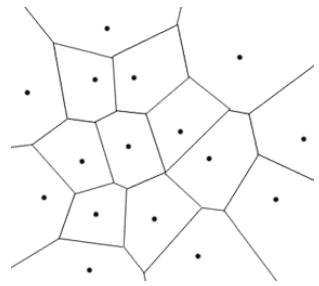
\includegraphics{../Voronoi/figures/fig1.eps}}
\end{center}


%=====================================================================
\section{Definitions}

Given a set of $S$ points $p_1, p_2, \ldots, p_n$ in the plane, a {\bf
Voronoi diagram} divides the plane into $n$ {\bf Voronoi regions} with
the following properties:
\begin{itemize}
\item Each point $p_i$ lies in exactly one region.

\item If a point $q \notin S$ lies in the same region as $p_i$, then
the Euclidian distance from $p_i$ to $q$ will be shorter than the
Euclidian distance from $p_j$ to $q$, where $p_j$ is any other point
in $S$.
\end{itemize}

The points $p_1, \ldots, p_n$ are called {\bf Voronoi sites}.  The
Voronoi diagram for two sites $p_i$ and $p_j$ can be easily
constructed by drawing the perpendicular bisector of line segment
$\overline{p_i p_j}$.

\begin{center}
\scalebox{0.75}{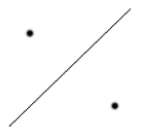
\includegraphics{../Voronoi/figures/fig2.eps}}
\end{center}

Such a diagram would consist of two unbounded Voronoi regions, denoted
$V(p_i)$ and $V(p_j)$.  In general, a Voronoi region $V(p_i)$ is
defined as the intersection of $n-1$ half-planes formed by taking the
perpendicular bisector of the segment $\overline{p_i p_j}$ for all
$p_j \in S$ where $i \neq j$.
\[ V(p_i) = H(p_i p_1) \ \cap H(p_i p_2) \ \cap \ldots \cap
H(p_i p_n) \]

\begin{center}
\scalebox{0.75}{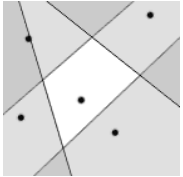
\includegraphics{../Voronoi/figures/fig3.eps}}
\end{center}

In this notation, $H(p_i p_j)$ refers to the half-plane formed by
taking the perpendicular bisector of $\overline{p_i p_j}$.  We know
that the intersection of any number of half-planes forms a convex
region bounded by a set of connected line segments. These line
segments form the boundaries of Voronoi regions and are called {\bf
Voronoi edges}.  The endpoints of these edges are called {\bf Voronoi
vertices}.

%=====================================================================
\section{Properties of Voronoi Diagrams}

\begin{itemize}
\item The number of Voronoi vertices is at most $2n - 5$.

\item The number of Voronoi edges is at most $3n - 6$.

\item Assuming {\em general position}\footnote{In this case, general
position implies that no four points will lie on the same circle.},
each Voronoi vertex is the common intersection point of exactly three
edges.

\item If site $p_i \in S$ is the nearest neighbor of site $p_j \in S$,
then the Voronoi regions $V(p_i)$ and $V(p_j)$ will share a common
edge.

\item Region $V(p)$ is unbounded iff $p$ is an extreme point of $S$.
That is, $p$ will be part of the convex hull of $S$.
\end{itemize}

Given a triangle $\triangle abc$, the perpendicular bisector of each
edge will intersect at a common point $q$ called the {\bf
circumcenter}.  The circumcenter is equi-distant from points $a,b,c$
and these points all lie on a circle with $q$ as its center.  This
circle is called the {\bf circumcircle} for triangle $\triangle abc$.

\begin{center}
\scalebox{0.75}{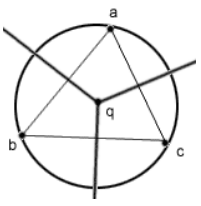
\includegraphics{../Voronoi/figures/fig4.eps}}
\end{center}

If a circumcircle is empty in its interior then, in a Voronoi diagram:
\begin{itemize}
\item $a,b,c$ would be Voronoi sites
\item $q$ would be a Voronoi vertex
\item The perpendicular bisectors of $\triangle abc$ would be Voronoi
edges.
\end{itemize}


%=====================================================================
\section{Delaunay Triangulation}

\begin{center}
\framebox{\scalebox{0.4}{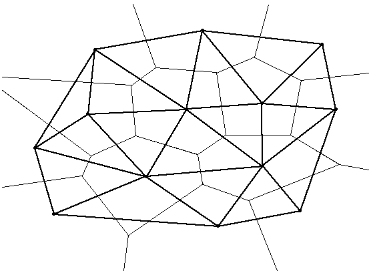
\includegraphics{../Voronoi/figures/fig8.eps}}} \\
\end{center}
A Delaunay Triangulation is a dual of a Voronoi diagram.  In a
Delaunay Triangulation two Voronoi sites are connected by an arc
iff $V(p_i)$ and $V(p_j)$ are bounded by a common Voronoi edge.  A
Delaunay Triangulation has the following properties:
\begin{itemize}
\item No two edges of the triangulation intersect in their interiors.
\item For all triangles $\triangle t$ of a triangulation, the
circumcircle for $\triangle t$ must be empty in its interior.  That
is, no Voronoi sites will lie inside the circumcircle for $\triangle
t$. 
\end{itemize}

%=====================================================================
\section{Constructing Voronoi Diagrams}

%---------------------------------------------------------------------
\subsection{Naive Approach}

A naive approach to construct of a Voronoi diagram is to determine the
region for each site, one at a time.  Since each region is the
intersection of $n-1$ half-planes, we can use an $O(n \log n)$
half-plane intersection algorithm to determine this region.  Repeating
for all $n$ points, we have an $O(n^2 \log n)$ algorithm.

%---------------------------------------------------------------------
\subsection{Divide and Conquer}

To construct a Voronoi diagram using the divide and conquer method,
first partition the set of points $S$ into two sets $L$ and $R$ based
on x-coordinates.  Next, construct the Voronoi diagrams for the left
and right subset Vor($L$) and Vor($R$).  Finally, merge the two
diagrams to produce Vor($S$).  If the merge step can be carried out in
linear time, then the construction of Vor($S$) can be accomplished in
$O(n \log n)$ time.


A Voronoi region is unbounded if and only if its site is an extreme
point (i.e. on the convex hull).  Note that as we compute the Voronoi
diagram for each subset, we can also compute the convex hull without
aversely affecting the time complexity.  We use this fact in the merge
step to find a starting point to {\em stitch} together the left and
right sub-diagrams. The merge algorithm works as follows:

\parbox{4.5in}{
\hrulefill \\
{\bf VORONOI\_MERGE} ($L$, $R$)
\begin{enumerate}

\item Find bridges to merge the convex hulls, CH($L$) and CH($R$).

\item Suppose the bottom bridge connects points $p \in L$ and $q \in
R$.
 \item Start with the perpendicular bisector of the bottom bridge
$\overline{pq}$.

\item Trace this bisector from $-\infty$ until it hits a Voronoi edge.

\item If the edge belongs to a Voronoi region from a point in $L$,
call this point $p$ and proceed upwards along the perpendicular
biscector of $\overline{pq}$.

\item Otherwise, if the edge belongs to a Voronoi region from a point
in $R$, call this point $q$ and proceed upwards along the
perpendicular bisector of $\overline{pq}$.

\item Repeat this process until the algorithm passes through the upper
bridge.

\item Finally, trim the left and right diagrams.
\begin{enumerate}
\item If an intersected edge belongs to the left diagram, discard the
section of the edge to the right of the intersection point. 
\item Likewise, if an intersected edge belongs to the right diagram, 
discard the section of the edge to teh left of the intersection point.
\end{enumerate}
\end{enumerate}
\hrulefill}

\begin{center}
\framebox{\scalebox{0.5}{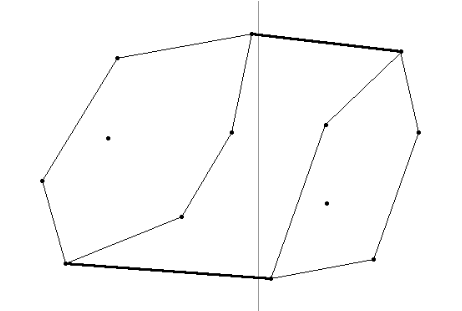
\includegraphics{../Voronoi/figures/fig-hull1.eps}}} \\
{\em
Step 1: Compute the convex hull for the left and right set of points\\
and find the upper and lower bridges.}
\vfill

\framebox{\scalebox{0.5}{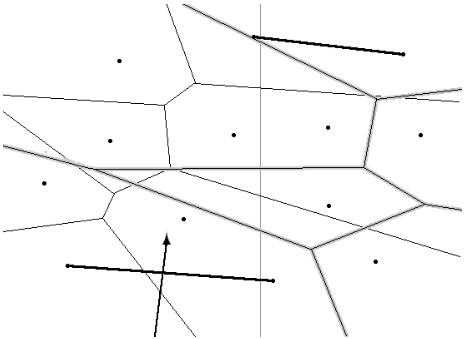
\includegraphics{../Voronoi/figures/fig-hull2.eps}}} \\
{\em Step 2: Trace the perpendicular bisector of the lower bridge from
$ - \infty$ and find the lowest intersection point with an edge of the
left or right Voronoi diagram.  In this figure, the left and right
Voronoi diagrams are shown overlaid on top of one another.  The edges
of the right diagram are highlighted with a grey border.  }

\framebox{\scalebox{0.5}{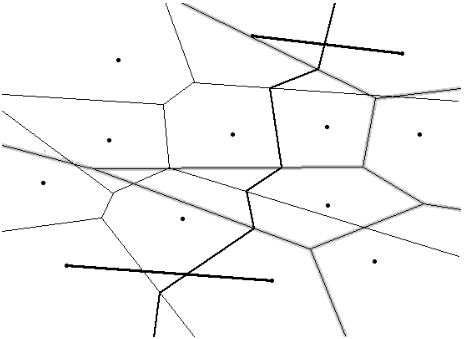
\includegraphics{../Voronoi/figures/fig-hull3.eps}}} \\ {\em
Step 3: Working upward, find the stitch.  At every new intersection of
the stitch and a Voronoi edge, recalculate the perpendicular
bisector.  Continue until the stitch crosses the upper bridge, and
there are no remaining intersections. }
\vfill

\framebox{\scalebox{0.5}{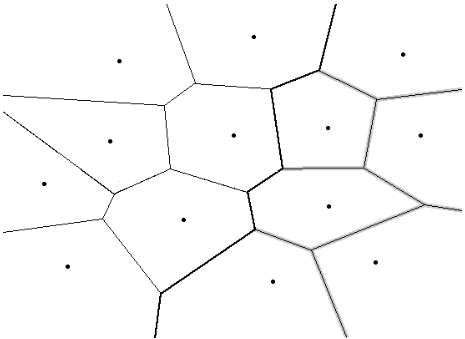
\includegraphics{../Voronoi/figures/fig-hull4.eps}}} \\
{\em Step 4: Trim the edges to complete the diagram.  Remove
everything from the left diagram that falls to the right of the
stitch.  Likewise, remove everything from the right diagram that falls
to the left of the stitch. }
\end{center}

%---------------------------------------------------------------------
\subsection{Sweep Line}

Given a set of points $p_1...p_n$ in the plane, we want to construct their 
voronoi diagram by sweeping a horizontal line across the points, keeping track 
of what was seen along the way.  In order to do this, we need to use an 
additional strategy involving parabolas.  Parabolas are useful in this 
sweep line problem because for any point $p_i$, there is a parabola separating 
$p_i$ from the sweep line in such a way that every point on the parabola is 
equidistant from both p and the sweep line.  Thus, when the sweep line reaches
a new point $p_j$, we will know, based on the parabola associated with each point,
what the midpoint is between $p_i$ and $p_j$.


Our algorithm will sweep a horizontal line from bottom to top, creating
a parabola for every point such that for any state of the sweep line, 
every point is the focus of its parabola, and the directrix of the parabola 
is the sweep line itself.  As seen in the figure below, the parabola for a 
particular site becomes wider as the sweep line continues its advance 
towards the top of the plane.


\begin{center}
\scalebox{0.75}{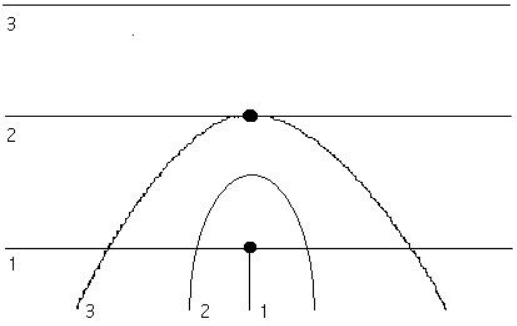
\includegraphics{../Voronoi/figures/fig5.eps}}
\end{center}


At any stage in the process, the algorithm resembles what we see below.
Above the sweep line is a set of unvisited sites, and every site below
the sweep line has, by an invariant of our algorithm, been visited already.  
The arcs closest to the sweep line create a ``wavefront,'' blocking other arcs
from view.  The points in the wavefront where arcs meet are called
break points, and we note that each break point is equidistant from its 
corresponding sites.  Every point surpassed by the wavefront is already known
to belong to a specific voronoi region.

\begin{center}
\scalebox{0.75}{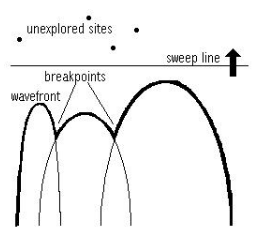
\includegraphics{../Voronoi/figures/fig6.eps}}
\end{center}


Consider the following observations:
\begin{enumerate}
\item As the sweep progresses, a new arc (of some parabola) is added to the
wavefront only when the sweep line touches some site.  This is called a 
$site$ $event$.

\item The only way that an arc can disappear from the wavefront is when two 
other adjacent arcs intersect it at a common point.  We call this a 
$circle$ $event$.
\end{enumerate}


\subsubsection{Data Structures}
Because we are interested in both site events and circle events, we will use
two data structures to store the information retrieved throughout the process.
The first data structure will be a balanced binary tree $T$ used to store
the wavefront.  Leaves of the tree will be the arcs making up the wavefront,
and the internal nodes of $T$ will be the breakpoints (intersections of arcs).

We will need the capability of performing the following operations on $T$:\begin{description}

\item[Insertions] When a new arc is added to the wavefront, we must insert it
into tree $T$.

\item[Deletions] When an arc becomes invisible to the sweep line it is no
longer a part of the wavefront and we must delete it from the tree.

\item[Search] For any vertical line we want to know which arc it
intersects

\end{description}


The second data structure we wish to use is a priority queue $Q$ to store the
events encountered.  The operations we would like to use are the following:\begin{description}

\item[Insert] We would like to be able to insert new events as they are found
in the process.

\item[Delete] After processing an event, it is no longer needed and we must
delete it from the queue.

\item[Successor] After an event is fully processed, we must process the next
 event in the queue based on y-coordinate.

\end{description}



\subsubsection{Complexity}

Notice that in the worst case, there are 2n-1 arcs on the wavefront at any
time (this occurs when every arc on the wavefront but one is split by another
wavefront arc).  Thus the balanced tree contains $O(n)$ elements.
Because each of the operations we wish to perform on $T$ takes no more than
$O(\log n)$ time and there are never more than $O(n)$ elements in the tree,
every operation of the wavefront status data structure is bounded by $O(\log n)$.

We note that circle events can only occur with three consecutive arcs.  Thus,
in a queue with at most n sites there are never more than n-2 circle events.  
Again our queue has $O(n)$ elements and so each of the operations takes no more
than $O(\log n)$ time.

Because there is a constant number of site events in $Q$ and each operation
takes a constant amount of time, we see that like the divide and conquer 
algorithm, this sweep line algorithm for determining the voronoi diagram 
over a set of n points runs in $O(n \log n)$ time.

\begin{center}
\scalebox{0.75}{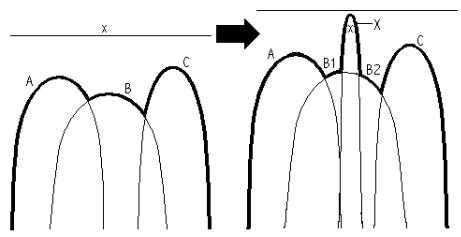
\includegraphics{../Voronoi/figures/fig7.eps}}
\end{center}

\parbox{4.5in}{
\hrulefill \\
{\bf VORONOI\_SWEEP} ({\sl P})\newline
{\sl Input.} A set $P=(p_1,p_2,...,p_n)$ of points in the plane.\newline
{\sl Output.} The Voronoi diagram Vor($P$).
\begin{enumerate}

\item Initialize a priority queue $Q$ with site events sorted by increasing
x-coordinate; initialize an empty status structure $T$

\item While $Q$ is nonempty:

\begin{enumerate}

\item Pop the next event $q$ off of $Q$ (smallest y-coordinate)

\item If $q$ is a site event X:

\begin{enumerate}

\item If $T$ is empty then insert $q$ into $T$ and return.  Otherwise
follow steps ii through iv.

\item Find the arc $B$ intersected by the parabola $X$ created from the 
sweep line and site x. (see diagram above)

\item Insert new parabola into $T$ and split the parabola ($B$) that it 
intersects into two pieces.  Rebalance $T$ if necessary.

\item Update $Q$ by deleting the circle event that is no longer possible based
on the slice through the wavefront ($A$-$B$-$C$), and by inserting the three 
newly possible circle events created by the new site event ($A$-$B1$-$X$, 
$B1$-$X$-$B2$, $X$-$B2$-$C$).

\end{enumerate}

\item If $q$ is a circle event ($x$: $A B x D E \rightarrow A B D E$):

\begin{enumerate}

\item Record the voronoi vertex.

\item Delete the arc that disappeared from $T$.

\item Update $Q$ by deleting the three now impossible circle events ($A$-$B$-$x$,
$B$-$x$-$D$, $x$-$D$-$E$) and inserting the two newly possible circle events 
$A$-$B$-$D$, $B$-$D$-$E$).

\end{enumerate}

\end{enumerate}

\end{enumerate}
\hrulefill}

%---------------------------------------------------------------------
\subsection{Conclusion}

It is interesting to note that the problem of sorting n numbers can be
reduced to the problem of constructing voronoi diagrams.  This means that
depite our efforts to find a voronoi diagram algorithm more efficient
than the two described above (each of which run in $O(n \log n)$ time), there 
is no such algorithm to be found.

\input{postamble}
